\subsection{Evaluation}

A useful evaluation locates the failure: unreadable input, missing evidence, unsupported interpretation or incorrect computation. One answer score cannot distinguish these causes. We organize benchmarks by the evidence they expose, then separate four observable properties of a document-QA response.

\subsubsection{Four Checks on One Answer}

Figure~\ref{fig:validation_cases} contrasts responses to the same source. A correct number can accompany the wrong citation; a relevant citation can accompany an invented explanation; and the correct cells can still be combined with faulty arithmetic. Evaluation should preserve these distinctions rather than collapse every response into a single success flag.

\begin{figure*}[tp]
\centering
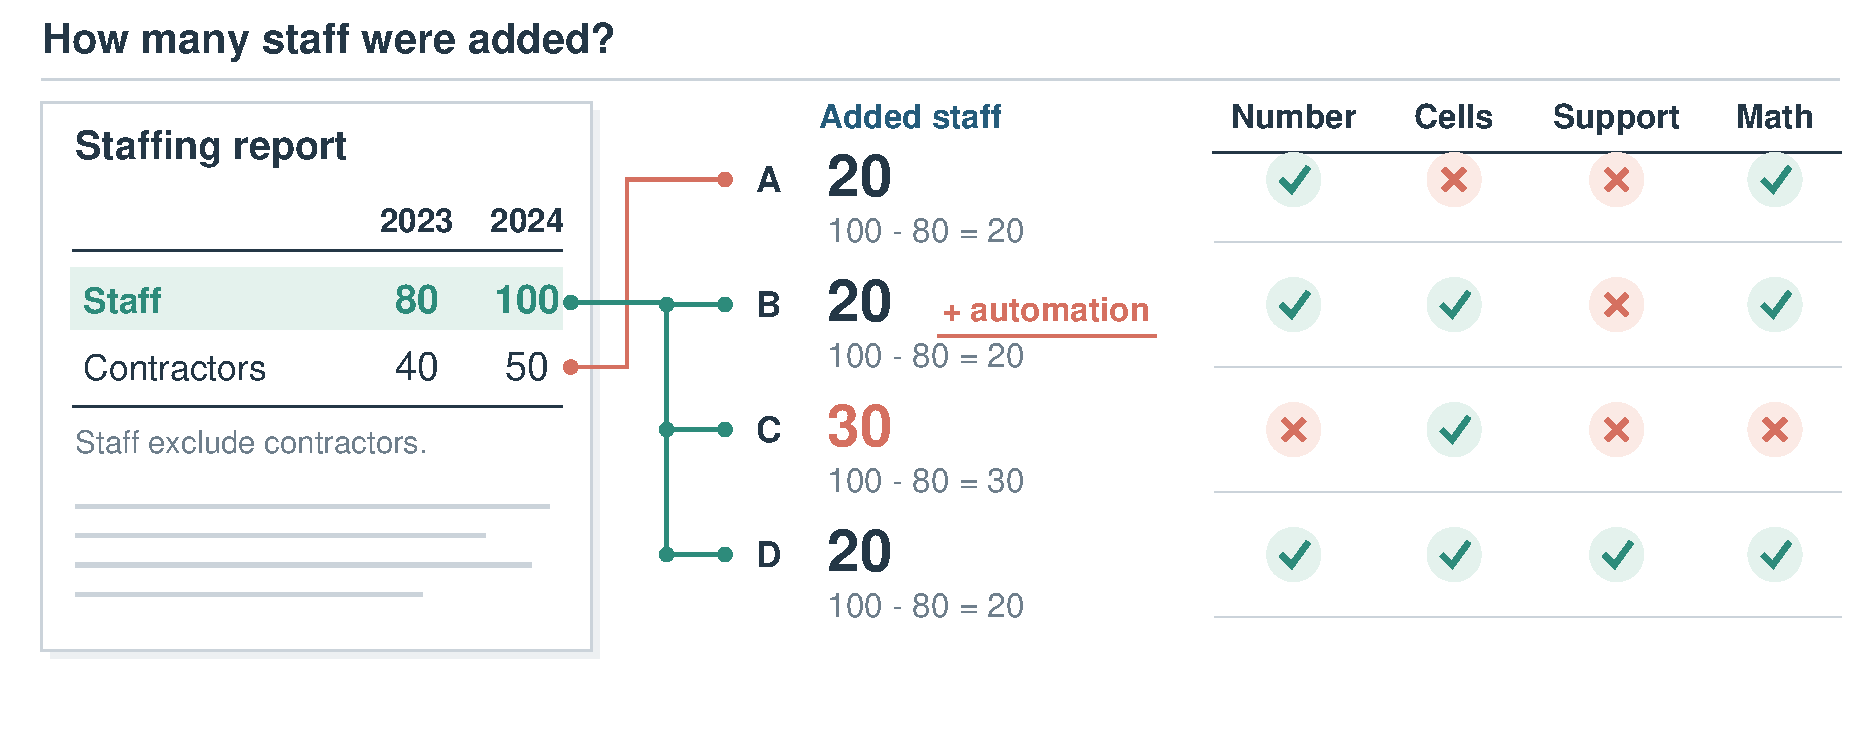
\includegraphics[width=\textwidth]{figs_by_qixingyu/fig14.pdf}
\caption{Constructed response traces separate numeric agreement, evidence localization, source support and arithmetic. The examples illustrate diagnostic outcomes, not measured model scores.}
\label{fig:validation_cases}
\end{figure*}

\textbf{Answer correctness} concerns the requested result and its unit. Exact match tests normalized string identity; token F1 measures overlap; ANLS uses normalized edit distance with the benchmark's threshold. These metrics suit different answer forms and should not be averaged across datasets as interchangeable percentages. For open-ended answers, the judge model, prompt and a human-audited sample help reveal whether fluent paraphrases or unsupported additions are being rewarded.

\textbf{Evidence localization} concerns the selected page, passage, region or cell. Recall measures whether required evidence is present; ranking metrics such as nDCG and MRR also consider its position. Gold-page experiments isolate the reader, whereas end-to-end retrieval experiments include evidence selection. Both are useful, but answer scores obtained with gold evidence should be reported separately from scores that require searching a collection.

\textbf{Source support} asks whether the cited material justifies the complete answer, including qualifications and explanations. A correct numerical component does not support an additional causal claim. Equivalent evidence may occur in several locations, so annotation should allow valid alternatives. Support is also distinct from causal faithfulness: establishing whether the model actually relied on the cited source requires interventions such as removing or substituting that evidence, not just checking the displayed citation.

\textbf{Execution correctness} asks whether the declared operation ran correctly on the supplied inputs. A Python or SQL result can verify arithmetic while using the wrong year, unit or table. It should therefore be paired with localization and semantic checks on those inputs. For multi-step questions, retain the intermediate values and their source locations so that a computational error can be separated from a parsing or planning error.

\subsubsection{Choose Benchmarks by Capability}

Table~\ref{tab:benchmark_capabilities} provides a compact selection map. The rows differ in task scope, evidence annotation and answerability; they do not form a common leaderboard. A page-reading benchmark is a weak test of collection search, while a retrieval benchmark alone does not test whether the final explanation is supported.

\begin{table*}[tp]
\centering
\small
\setlength{\tabcolsep}{3pt}
\renewcommand{\arraystretch}{1.15}
\begin{tabularx}{\textwidth}{@{}p{0.20\textwidth}p{0.21\textwidth}Xp{0.19\textwidth}@{}}
\toprule
Resource & Scope & Released supervision & Main metrics \\
\midrule
DocVQA~\cite{docvqa2020} & One page & Answer strings & ANLS \\
InfographicVQA~\cite{infographicvqa2021} & Infographic & Answers; categories & ANLS \\
QASPER~\cite{infoseekqa2021} & Scientific paper & Answers + evidence; unanswerable & Answer / Evidence F1 \\
SlideVQA~\cite{slidevqa2023} & Slide deck & Answers + pages + expressions & QA / evidence EM, F1 \\
DUDE~\cite{dude2023} & Multiple pages & Multiple answer types; unanswerable & ANLS-based scoring \\
MMLongBench-Doc~\cite{mmlongbenchdoc2024} & Long visual PDF & Answers + source pages; unanswerable & Answer F1 \\
ViDoRe (original)~\cite{faysse2024colpali} & Page retrieval & Relevant-page judgments & nDCG@5; Recall@K \\
CRAG~\cite{crag2024} & Factual RAG & Answers; invalid queries; graded responses & Accuracy; hallucination \\
\bottomrule
\end{tabularx}
\caption{Eight evaluation resources selected by task and released supervision. Evidence annotations are not necessarily provided to the tested reader; input access must be stated.}
\label{tab:benchmark_capabilities}
\end{table*}

For single-page reading, DocVQA emphasizes document text and layout, while InfographicVQA adds graphics and visual organization. The latter's first preprint appeared in 2021, before its WACV 2022 publication. Multi-page benchmarks expose a different difficulty: QASPER links answers to supporting paper content, and SlideVQA includes evidence pages and numerical expressions. These annotations enable diagnostics that answer strings alone cannot support, including whether the system found all necessary pages.

Long documents and collections separate context capacity from search quality. MMLongBench-Doc tests mixed visual evidence across long PDFs; ViDoRe tests query-to-page retrieval. Evaluating both can reveal whether a visual RAG pipeline fails before or after evidence reaches its reader. MultiHop-RAG adds another axis: composing support across more than one source~\cite{multihoprag2024}. A high single-page score provides little information about that composition step.

Domain and document quality should be selected deliberately. LegalBench-RAG focuses retrieval on legal material, while REAL-MM-RAG studies heterogeneous enterprise evidence~\cite{legalbenchragr2024,realmmrag2025}. M6Doc and RoDLA instead probe layout diversity and robustness~\cite{m6doc2023,rodla2024}. These resources answer different questions: domain retrieval can fail despite clean OCR, and degraded page structure can fail before retrieval begins. A practical evaluation combines the relevant stages rather than treating one benchmark as a universal proxy.

Answerability and freshness require separate cases. DUDE and QASPER include unanswerable questions; CRAG distinguishes accurate, hallucinated and missing responses. Dedicated unanswerability studies examine when a RAG system should decline~\cite{unanswerablerag2024}. FreshStack evaluates retrieval in a changing technical corpus~\cite{freshstack2025}. Report refusal together with coverage and error rate: a system that declines every difficult question can appear conservative while supplying little useful information.

\subsubsection{A Matched Comparison Protocol}

Match the document snapshot and split; raw images versus native text or supplied OCR; gold pages versus collection search; image resolution, crops and context budgets; model or API version; retrieval depth and tool limits. Include full-context and OCR-based controls where they receive equivalent information. Report answer and evidence metrics alongside ingestion cost, online latency and failed requests, with breakdowns for document length, scan quality, language and evidence modality. This protocol makes the comparison interpretable without turning every architectural change into a claim of general superiority.
